\newpage


\begin{center}
\newpage
\thispagestyle{plain}
\textbf{\Huge Capítulo 3}
\end{center}
\begin{center}
\textbf{\Huge Revisão da Literatura}
\end{center}
\noindent\makebox[\linewidth]{\rule{\textwidth}{1pt}} 
\begin{flushleft}
O Capítulo \ref{chapter:cap3-mapeamento-sistematico} apresenta uma revisão da literatura por meio do arcabouço teórico do estudo e um MS que busca responder as seguintes questões (Q):

\begin{itemize}
    \item[Q1 -] Que informação o corpo atual da literatura oferece com relação ao problema de pesquisa identificado?
    \item[Q2 -] Como DevOps está sendo aplicado no Processo de Produção de Software?
    \item[Q3 -] Como ocorre a implantação do DevOps no Processo de Produção de Software?
    \item[Q4 -] O processo de Produção de Software possui modelos de maturidade para implantação de DevOps?
\end{itemize}

Por fim, apresenta os trabalhos relacionados ao estudo e um comparativo dos estudos encontrados.
\end{flushleft}
\noindent\makebox[\linewidth]{\rule{\textwidth}{1pt}} 

Este capítulo encontra-se na fase de pesquisa descrita na imagem a seguir:
\begin{figure}[ht]
\centering
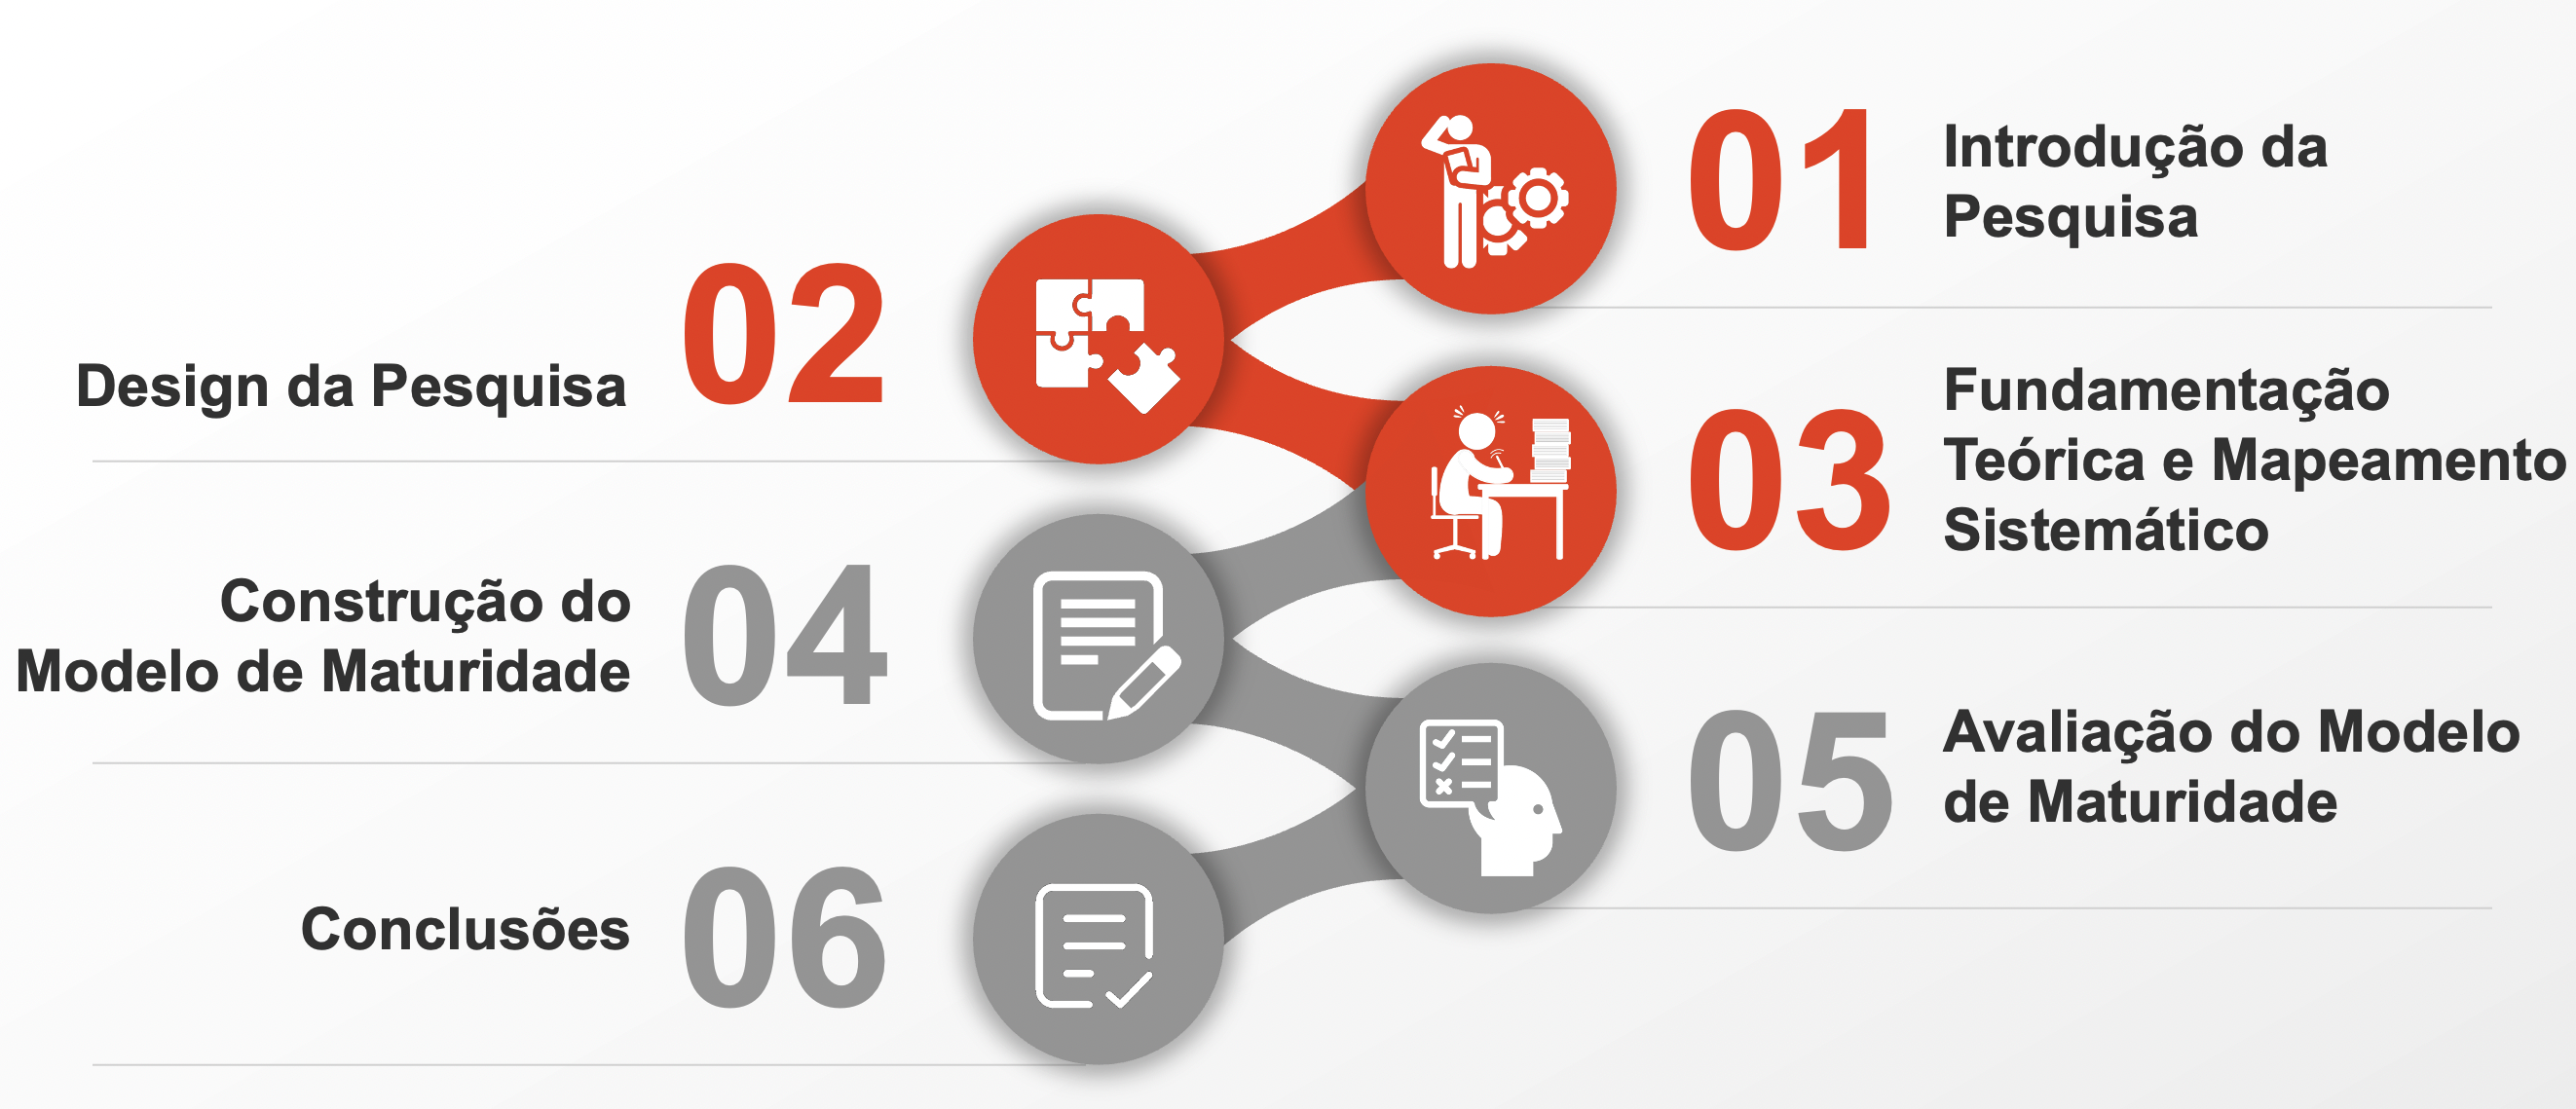
\includegraphics[width=15cm]{images/part-capitulo3.png}
\label{fig:metodologia-cap2}
\end{figure}